

\section{Toy Petri Net Example}
\label{appendix:toyPN}

Observe the toy Petri net in Fig.~\ref{fig:toyPN}.

\begin{figure}[H]
	\centering
	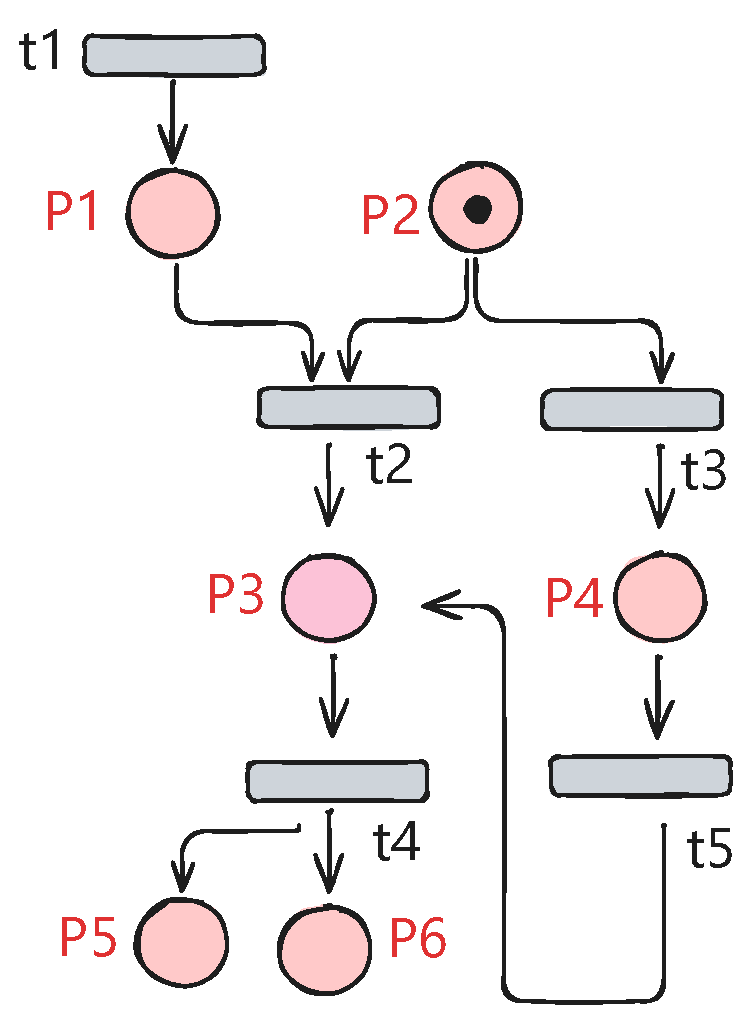
\includegraphics[width=0.3\textwidth]{plots/toy_PN_example.pdf}
	\caption{A toy Petri net.}
	\label{fig:toyPN}
\end{figure}



We formally define the net as follows:

 \(N=(P,T,\mathsf{pre},\mathsf{post},M_0)\) with
\[
P=\{P_1,P_2,P_3,P_4,P_5,P_6\},\quad
T=\{t_1,t_2,t_3,t_4,t_5\},
\]
and the flow functions $\mathsf{pre}$,$\mathsf{post}$ are given as
\[
\begin{array}{c|cccccc}
	& P_1 & P_2 & P_3 & P_4 & P_5 & P_6 \\ \hline
	\mathsf{pre}(t_1)  & 0 & 0 & 0 & 0 & 0 & 0 \\
	\mathsf{post}(t_1) & 1 & 0 & 0 & 0 & 0 & 0 \\ \hline
	\mathsf{pre}(t_2)  & 1 & 1 & 0 & 0 & 0 & 0 \\
	\mathsf{post}(t_2) & 0 & 0 & 1 & 0 & 0 & 0 \\ \hline
	\mathsf{pre}(t_3)  & 0 & 1 & 0 & 0 & 0 & 0 \\
	\mathsf{post}(t_3) & 0 & 0 & 0 & 1 & 0 & 0 \\ \hline
	\mathsf{pre}(t_4)  & 0 & 0 & 1 & 0 & 0 & 0 \\
	\mathsf{post}(t_4) & 0 & 0 & 0 & 0 & 1 & 1 \\ \hline
	\mathsf{pre}(t_5)  & 0 & 0 & 0 & 1 & 0 & 0 \\
	\mathsf{post}(t_5) & 0 & 0 & 1 & 0 & 0 & 0
\end{array}
\]
The initial marking is
\[
M_0 = (0,1,0,0,0,0)^\top 
\]

Differently put, there is a single token in place $P_2$.


\begin{itemize}
	\item An examples of a \emph{reachable} marking is
	\[
	M_f = (0,0,0,0,1,1)^\top,
	\]
	reached by the firing sequence
	\[
	M_0 \xrightarrow{t_1} M_1
	\xrightarrow{t_2} M_2
	\xrightarrow{t_4} M_f,
	\]
	where
	\[
	M_1 = (1,1,0,0,0,0)^\top,
	\quad
	M_2 = (0,0,1,0,0,0)^\top.
	\]
	\item An example of a \emph{non-reachable} marking is
	\[
	M_{nr} = (0,1,1,0,0,0)^\top.
	\]
	Since producing a token at \(P_3\) (via \(t_2\)) necessarily consumes the only token in \(P_2\), and no transition replenishes \(P_2\), then it is impossible for these two places to \textit{simultaneously} hold a single token in any reachable firing. However, we note that if the initial marking were 
	
	\[
	M_0' = (0,2,0,0,0,0)^\top,
	\]
	then marking $M_{nr}$ \textit{would have} been reachable, by firing a single transition $t_1$, followed by a single transition $t_2$.
\end{itemize}






%\newpage